\subsection{Message Passing Detector Design}

After OTFS demodulation, the receiver obtains the delay-Doppler observation vector \(\mathbf{y}\). Because the channel is time-varying and multipath, each received delay-Doppler sample may contain contributions from several transmitted symbols. A direct exhaustive search over all possible transmitted symbol vectors would be computationally impractical. Therefore, the baseline OTFS receiver uses a message passing detector to estimate the transmitted QAM symbols from the sparse delay-Doppler input-output model.

The detector used in this thesis follows the message passing structure commonly adopted for OTFS detection over sparse delay-Doppler channels. The same detector core is later reused for OTFS-IM. In the baseline OTFS case, the detector output is used to form hard QAM symbol decisions. In the OTFS-IM case, the probability output of the same detector is further processed to detect both active positions and QAM symbols, as discussed in Chapter 4.

\subsubsection{Motivation for Message Passing Detection}

From Section 3.5, the equivalent delay-Doppler input-output relation can be written as
\begin{equation}
    \mathbf{y}
    =
    \mathbf{H}_{\mathrm{DD}}\mathbf{x}
    +
    \mathbf{w}.
\end{equation}
The matrix \(\mathbf{H}_{\mathrm{DD}}\) is sparse because the channel contains only a limited number of delay-Doppler paths. This means that each received symbol is mainly affected by a small subset of transmitted symbols, rather than by all \(MN\) transmitted symbols.

This sparse structure makes message passing suitable for OTFS detection. Instead of solving the full linear system using a dense matrix inversion, the detector iteratively exchanges probability information between received observation nodes and transmitted symbol nodes. The algorithm estimates the probability that each transmitted symbol belongs to each constellation point, and then makes a hard decision after the probabilities converge or the maximum number of iterations is reached.

\begin{figure}[H]
    \centering
    \begin{tikzpicture}[
        startstop/.style={
            rectangle,
            rounded corners,
            draw,
            thick,
            align=center,
            text width=5.4cm,
            minimum height=0.72cm,
            font=\footnotesize,
            inner sep=4pt
        },
        io/.style={
            trapezium,
            trapezium left angle=70,
            trapezium right angle=110,
            draw,
            thick,
            align=center,
            text width=5.2cm,
            minimum height=0.72cm,
            font=\footnotesize,
            inner sep=4pt
        },
        process/.style={
            rectangle,
            draw,
            thick,
            align=center,
            text width=5.9cm,
            minimum height=0.72cm,
            font=\footnotesize,
            inner sep=4pt
        },
        decision/.style={
            diamond,
            draw,
            thick,
            align=center,
            text width=2.7cm,
            aspect=1.85,
            font=\footnotesize,
            inner sep=1pt
        },
        arrow/.style={
            ->,
            thick
        }
    ]

        \node[io] (input) at (0,0) {Input \(\mathbf{y}\), channel taps, channel gains, \(\sigma^2\)};
        \node[process] (init) at (0,-1.50) {Initialize candidate alphabet and uniform probabilities};
        \node[process] (meanvar) at (0,-3.00) {Observation-node update: compute interference mean and variance};
        \node[process] (prob) at (0,-4.50) {Variable-node update: compute likelihoods and symbol probabilities};
        \node[process] (damp) at (0,-6.00) {Apply damping to stabilize probability updates};
        \node[decision] (conv) at (0,-8.05) {Converged or max iterations?};
        \node[startstop] (hard) at (0,-10.35) {Hard decision and final probability output};

        \draw[arrow] (input.south) -- (init.north);
        \draw[arrow] (init.south) -- (meanvar.north);
        \draw[arrow] (meanvar.south) -- (prob.north);
        \draw[arrow] (prob.south) -- (damp.north);
        \draw[arrow] (damp.south) -- (conv.north);
        \draw[arrow] (conv.south) -- node[right, font=\footnotesize, pos=0.45] {Yes} (hard.north);
        \draw[arrow] (conv.east) -- ++(2.25,0) |- node[pos=0.25, right, font=\footnotesize] {No} (meanvar.east);

    \end{tikzpicture}
    \caption{Operational flow of the message passing detector}
    \label{fig:mp_detector_flow}
\end{figure}

Figure~\ref{fig:mp_detector_flow} summarizes the operational flow of the detector. The algorithm starts with uniform symbol probabilities, repeatedly refines the interference statistics and symbol probabilities, and stops when the probability decisions become sufficiently reliable or when the iteration limit is reached.

\subsubsection{Sparse Factor-Graph Interpretation}

The message passing detector can be interpreted using a factor graph. In this graph, variable nodes represent transmitted symbols, while observation nodes represent received delay-Doppler samples. An edge exists between a variable node and an observation node if the corresponding transmitted symbol contributes to that received sample through one of the channel taps.

\begin{figure}[H]
    \centering
    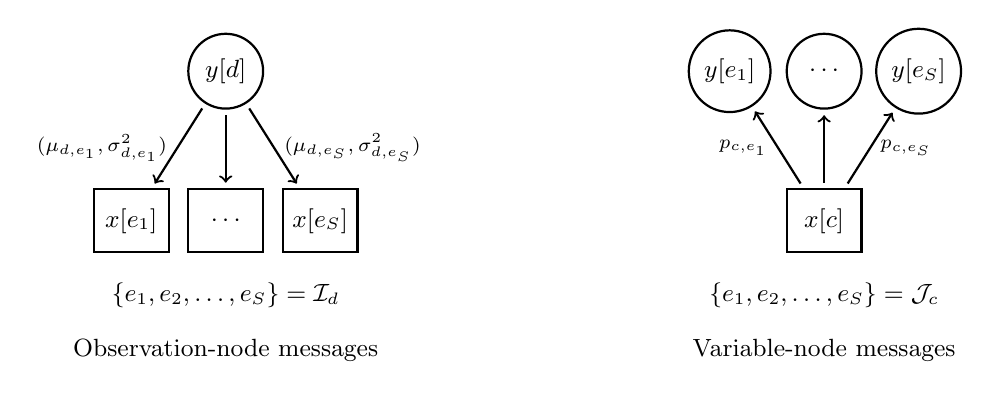
\begin{tikzpicture}[
        obsnode/.style={
            circle,
            draw,
            thick,
            align=center,
            minimum size=0.95cm,
            font=\small
        },
        varnode/.style={
            rectangle,
            draw,
            thick,
            align=center,
            minimum width=0.95cm,
            minimum height=0.8cm,
            font=\small
        },
        arrow/.style={
            ->,
            thick,
            shorten >=2pt,
            shorten <=2pt
        }
    ]

        % Observation-node messages
        \node[obsnode] (yd) at (-3.8,0.3) {\(y[d]\)};
        \node[varnode] (xe1) at (-5.0,-1.6) {\(x[e_1]\)};
        \node[varnode] (xe2) at (-3.8,-1.6) {\(\cdots\)};
        \node[varnode] (xes) at (-2.6,-1.6) {\(x[e_S]\)};

        \draw[arrow] (yd) -- node[left, font=\scriptsize, pos=0.52]
            {\((\mu_{d,e_1},\sigma^2_{d,e_1})\)} (xe1);
        \draw[arrow] (yd) -- (xe2);
        \draw[arrow] (yd) -- node[right, font=\scriptsize, pos=0.52]
            {\((\mu_{d,e_S},\sigma^2_{d,e_S})\)} (xes);

        \node[align=center, font=\small] at (-3.8,-2.55)
            {\(\{e_1,e_2,\ldots,e_S\}=\mathcal{I}_d\)};
        \node[align=center, font=\small] at (-3.8,-3.25)
            {Observation-node messages};

        % Variable-node messages
        \node[varnode] (xc) at (3.8,-1.6) {\(x[c]\)};
        \node[obsnode] (ye1) at (2.6,0.3) {\(y[e_1]\)};
        \node[obsnode] (ye2) at (3.8,0.3) {\(\cdots\)};
        \node[obsnode] (yes) at (5.0,0.3) {\(y[e_S]\)};

        \draw[arrow] (xc) -- node[left, font=\scriptsize, pos=0.50]
            {\(p_{c,e_1}\)} (ye1);
        \draw[arrow] (xc) -- (ye2);
        \draw[arrow] (xc) -- node[right, font=\scriptsize, pos=0.50]
            {\(p_{c,e_S}\)} (yes);

        \node[align=center, font=\small] at (3.8,-2.55)
            {\(\{e_1,e_2,\ldots,e_S\}=\mathcal{J}_c\)};
        \node[align=center, font=\small] at (3.8,-3.25)
            {Variable-node messages};

    \end{tikzpicture}
    \caption{Observation-node and variable-node messages in the MP detector}
    \label{fig:mp_factor_graph}
\end{figure}

Figure~\ref{fig:mp_factor_graph} illustrates the two types of messages exchanged in the MP detector. An observation node \(y[d]\) sends interference statistics, represented by the mean and variance pair \((\mu_{d,e},\sigma^2_{d,e})\), to its neighboring variable nodes. Conversely, a variable node \(x[c]\) sends probability messages \(p_{c,e}\) to the observation nodes connected to it. The neighbor sets \(\mathcal{I}_d\) and \(\mathcal{J}_c\) are determined by the delay taps, Doppler taps, and channel coefficients. Since the number of paths is small, each node is connected only to a limited number of neighboring nodes. This locality is the main reason why message passing can reduce the detection complexity.

\begin{algorithm}[H]
    \caption{Message passing detector for OTFS symbol detection}
    \label{alg:mp_detector}
    \begin{algorithmic}[1]
        \REQUIRE Received delay-Doppler vector \(\mathbf{y}\), delay taps, Doppler taps, channel coefficients, noise variance \(\sigma^2\), candidate alphabet \(\mathcal{A}_{0}\)
        \ENSURE Hard symbol estimate \(\widehat{\mathbf{x}}\) and final probability map
        \STATE Vectorize the received grid as \(\mathbf{y}=\mathrm{vec}(\mathbf{y}_{\mathrm{DD}})\)
        \STATE Initialize all symbol probabilities uniformly over \(\mathcal{A}_{0}\)
        \FOR{\(i=1\) to \(N_{\mathrm{ite}}\)}
            \STATE For each observation-symbol connection, compute the effective channel coefficient from the delay and Doppler taps
            \STATE Compute the interference mean by excluding the candidate symbol being updated
            \STATE Compute the interference variance and add the noise variance \(\sigma^2\)
            \STATE Evaluate the likelihood of every candidate symbol in \(\mathcal{A}_{0}\)
            \STATE Normalize the likelihoods to obtain updated symbol probabilities
            \STATE Apply damping between the new probabilities and the previous probabilities
            \STATE Compute the convergence rate from the maximum probability at each symbol position
            \IF{all symbol positions are reliable or the convergence rate degrades}
                \STATE Stop the iteration
            \ENDIF
        \ENDFOR
        \STATE Select the symbol with the largest final probability at each position
        \RETURN \(\widehat{\mathbf{x}}\) and the final probability map
    \end{algorithmic}
\end{algorithm}

Algorithm~\ref{alg:mp_detector} presents the computational order of the detector. The most important idea is that the detector does not decide symbols immediately after OTFS demodulation. Instead, it repeatedly estimates the interference caused by neighboring delay-Doppler symbols and uses this estimate to refine the probability of each candidate symbol.

\subsubsection{Algorithmic Complexity Interpretation}

The advantage of message passing becomes clearer when it is compared with an exhaustive detector. If all \(MN\) transmitted OTFS symbols were detected jointly, the search space would grow as \(|\mathcal{A}|^{MN}\), where \(|\mathcal{A}|\) is the constellation size. This is impossible even for moderate frame sizes. For the baseline setup in this thesis, \(MN=120\), so a full joint search over 4-QAM candidates would require \(4^{120}\) possible symbol vectors. This number is far beyond practical simulation or implementation.

The MP detector avoids this full search by using the sparse delay-Doppler channel structure. Since each received observation is connected only to a limited number of transmitted symbols, the detector updates probabilities locally rather than globally. If the number of channel paths is \(P\), the number of detector iterations is \(N_{\mathrm{ite}}\), and the candidate alphabet size is \(|\mathcal{A}_{0}|\), a useful high-level complexity description is
\begin{equation}
    \mathcal{O}
    \left(
    N_{\mathrm{ite}}
    MN
    P
    |\mathcal{A}_{0}|
    \right).
    \label{eq:mp_complexity_order}
\end{equation}
This expression is not intended to count every arithmetic operation exactly. Its purpose is to show the scaling behavior: the computational effort grows approximately linearly with the number of delay-Doppler resource elements, the number of channel paths, the number of iterations, and the number of candidate symbols.

This complexity interpretation also explains why the same detector can be reused for OTFS-IM. In OTFS-IM, the alphabet is extended by adding the inactive symbol \(0\). Therefore, the detector does not need a different factor-graph structure. It only evaluates one additional candidate state per resource element. The more difficult OTFS-IM operation is not the MP update itself, but the block-wise interpretation of the resulting probability map, which is developed in Chapter 4.

From a reporting perspective, this distinction is important. The MP detector provides a soft reliability profile over the delay-Doppler grid. The later OTFS-IM receiver then uses this reliability profile to decide which positions are active. Therefore, the detector is not only a symbol estimator; it is also the probability engine that enables index detection.

\subsubsection{Role of Damping and Stopping in the Iterative Process}

The damping factor is included because probability messages in a loopy factor graph can oscillate between iterations. In an ideal tree-structured factor graph, messages can converge in a finite number of passes. The OTFS detection graph, however, contains cycles because several transmitted symbols can affect several received observations through different delay-Doppler shifts. In this case, updating probabilities too aggressively may cause the detector to overreact to an unreliable intermediate estimate.

Damping reduces this problem by mixing the newly computed probability with the previous probability. A large damping factor gives more weight to the new likelihood information and can lead to faster convergence when the observation is reliable. A smaller damping factor makes the detector more conservative and can improve stability when the received observation is noisy or when the interference estimate is still inaccurate. The value \(\Delta=0.6\) used in the simulation therefore represents a compromise between convergence speed and numerical stability.

The convergence criterion is also important. The detector does not need to run the full number of iterations if most symbol probabilities have already become reliable. In this thesis, reliability is measured by checking whether the largest candidate probability at a symbol position exceeds a high threshold. If the maximum probability is close to one, the detector is confident about that symbol decision. If many positions remain uncertain, additional iterations may still improve the probability map.

However, more iterations do not always guarantee better BER. In a loopy message-passing detector, later iterations can sometimes reinforce an incorrect decision if the probability map becomes overconfident too early. For this reason, the stopping rule also monitors whether the convergence behavior is improving. The detector is therefore designed to stop when the probability map has become sufficiently reliable or when further iterations are unlikely to provide useful improvement.

\begin{table}[H]
\centering
\caption{Interpretation of key MP detector parameters.}
\label{tab:mp_detector_parameter_roles}
\begin{tabularx}{0.95\linewidth}{|p{3.0cm}|X|}
\hline
\textbf{Parameter} & \textbf{Role in the detector} \\
\hline
\(P\) & Number of channel paths; determines how many neighboring symbols contribute significantly to each observation. \\
\hline
\(|\mathcal{A}_{0}|\) & Number of candidate symbol states; includes QAM symbols and, for OTFS-IM reuse, the inactive zero state. \\
\hline
\(N_{\mathrm{ite}}\) & Maximum number of message-passing iterations; limits complexity and prevents endless updates. \\
\hline
\(\Delta\) & Damping factor; balances new probability information and previous messages to improve stability. \\
\hline
\(\sigma^2\) & Noise variance; affects the likelihood width and therefore the confidence of probability updates. \\
\hline
\end{tabularx}
\end{table}

Table~\ref{tab:mp_detector_parameter_roles} also shows why detector parameters must be reported together with BER results. If the number of iterations, damping factor, or noise normalization were changed, the detector output probabilities could change even under the same channel realization. Keeping these parameters fixed is therefore necessary for a fair comparison between baseline OTFS and OTFS-IM.

\subsubsection{Symbol Alphabet and Probability Initialization}

Let \(\mathcal{A}\) denote the QAM constellation alphabet. For baseline OTFS with 4-QAM, \(\mathcal{A}\) contains four constellation points. The detector estimates, for each transmitted symbol position, the probability that the symbol belongs to each element of the alphabet.

To make the detector reusable for both baseline OTFS and OTFS-IM, an extended candidate alphabet is defined as
\begin{equation}
    \mathcal{A}_{0}
    =
    \mathcal{A}
    \cup
    \{0\}.
\end{equation}
The zero symbol is included because the same detector is later used for OTFS-IM, where inactive positions correspond to zero-valued transmitted symbols. For the baseline OTFS discussion, the important point is that the detector produces symbol probabilities over the candidate alphabet. The probability output is then used either for direct hard QAM decisions in baseline OTFS or for block-wise index detection in OTFS-IM.

At the beginning of the algorithm, all symbol candidates are assigned equal probability:
\begin{equation}
    p_{c,d}^{(0)}(a_j)
    =
    \frac{1}{|\mathcal{A}_{0}|},
    \qquad
    a_j\in\mathcal{A}_{0}.
    \label{eq:mp_uniform_initialization}
\end{equation}
This initialization avoids biasing the first iteration toward any constellation point or inactive state.

\subsubsection{Observation-Node Mean and Variance Update}

Consider one received observation \(y[d]\) and one transmitted symbol \(x[c]\) connected to it. The received sample can be written as
\begin{equation}
    y[d]
    =
    H[d,c]x[c]
    +
    \sum_{e\in\mathcal{I}(d),\,e\neq c}
    H[d,e]x[e]
    +
    w[d],
    \label{eq:mp_observation_model}
\end{equation}
where \(\mathcal{I}(d)\) is the set of transmitted symbols connected to observation node \(d\). The summation term represents the interference caused by other connected symbols.

In message passing detection, this interference is approximated as a Gaussian random variable. Therefore, for each connected edge, the observation node computes the mean and variance of the interference using the current symbol probabilities. If \(p_{e,d}^{(i-1)}(a_j)\) is the probability from the previous iteration that \(x[e]=a_j\), the interference mean can be expressed as
\begin{equation}
    \mu_{d,c}^{(i)}
    =
    \sum_{e\in\mathcal{I}(d),\,e\neq c}
    \sum_{a_j\in\mathcal{A}_{0}}
    p_{e,d}^{(i-1)}(a_j)
    a_j
    H[d,e].
\end{equation}
The corresponding variance is
\begin{equation}
    \begin{aligned}
    \left(\sigma_{d,c}^{(i)}\right)^2
    &=
    \sum_{e\in\mathcal{I}(d),\,e\neq c}
    \Bigg(
    \sum_{a_j\in\mathcal{A}_{0}}
    p_{e,d}^{(i-1)}(a_j)
    |a_j|^2
    |H[d,e]|^2
    \\
    &\qquad
    -
    \left|
    \sum_{a_j\in\mathcal{A}_{0}}
    p_{e,d}^{(i-1)}(a_j)
    a_j
    H[d,e]
    \right|^2
    \Bigg)
    +
    \sigma^2.
    \end{aligned}
\end{equation}
These two quantities summarize the contribution of all interfering symbols except the candidate symbol currently being updated.

\subsubsection{Variable-Node Probability Update with Damping}

After the observation-node update, the detector updates the probability of each candidate symbol. For a candidate value \(a_j\), the likelihood is computed by comparing the received observation with the predicted contribution of \(a_j\), while treating the remaining interference as Gaussian. A compact likelihood expression is
\begin{equation}
    \xi^{(i)}(d,c,a_j)
    =
    \exp
    \left(
    -
    \frac{
    \left|
    y[d]
    -
    \mu_{d,c}^{(i)}
    -
    H[d,c]a_j
    \right|^2
    }{
    \left(\sigma_{d,c}^{(i)}\right)^2
    }
    \right).
\end{equation}
The probability of each candidate symbol is then updated using the product of the likelihoods from the connected observation nodes. This follows the standard message passing principle that a variable node combines information from its neighboring observation nodes.

For numerical stability, the probability update can be evaluated in the logarithmic domain. After the new probability is computed, damping is applied:
\begin{equation}
    p_{c,d}^{(i)}(a_j)
    =
    \Delta \widetilde{p}_{c,d}^{(i)}(a_j)
    +
    (1-\Delta)p_{c,d}^{(i-1)}(a_j),
    \label{eq:mp_damping}
\end{equation}
where \(\widetilde{p}_{c,d}^{(i)}(a_j)\) is the newly computed probability and \(\Delta\) is the damping factor. In the simulation, the damping factor is set to
\begin{equation}
    \Delta = 0.6.
\end{equation}
Damping prevents the probabilities from changing too aggressively between iterations. This helps stabilize the iterative detector, especially when the factor graph contains cycles.

\subsubsection{Hard Decision and Convergence Criterion}

At each iteration, the detector computes the final symbol probability for every transmitted position. The hard decision is obtained by selecting the candidate symbol with the largest probability:
\begin{equation}
    j^{\star}
    =
    \arg\max_{j}
    p_c(a_j).
\end{equation}
The detected symbol is then
\begin{equation}
    \widehat{x}[c] = a_{j^{\star}}.
    \label{eq:mp_hard_decision}
\end{equation}

The implementation also evaluates a convergence indicator. A symbol position is considered reliable if the maximum probability exceeds \(0.99\). The convergence rate is therefore computed as the fraction of symbol positions satisfying this condition:
\begin{equation}
    \eta^{(i)}
    =
    \frac{1}{MN}
    \sum_{c=1}^{MN}
    \mathbf{1}
    \left(
    \max_{a_j\in\mathcal{A}_{0}} p_c^{(i)}(a_j) > 0.99
    \right).
\end{equation}
If all positions become reliable, the detector stops early. Otherwise, the algorithm continues until the maximum number of iterations is reached. In the simulation, the maximum number of message passing iterations is
\begin{equation}
    N_{\mathrm{ite}} = 10.
\end{equation}

\subsubsection{Detector Input and Output Summary}

The detector takes the received delay-Doppler observation, the OTFS frame size, the QAM order, the delay and Doppler taps, the channel coefficients, and the noise variance as its main inputs. The received grid is first vectorized so that each delay-Doppler position can be treated as one variable node in the factor graph:
\begin{equation}
    \mathbf{y}_{v}
    =
    \mathrm{vec}\!\left(\mathbf{y}_{\mathrm{DD}}\right).
    \label{eq:mp_received_vectorization}
\end{equation}
The detector then initializes the probability map, iteratively updates the interference mean and variance, updates the symbol probabilities with damping, and finally returns both a hard symbol estimate and a final probability map. The hard estimate is denoted by \(\widehat{\mathbf{x}}\), while the final probability map is denoted by \(\mathbf{P}_{\mathrm{fin}}\).

For the baseline OTFS system, \(\widehat{\mathbf{x}}\) is used to recover the QAM symbols and compute the BER. For the OTFS-IM system in Chapter 4, \(\mathbf{P}_{\mathrm{fin}}\) becomes especially important because it provides the probability that each position is active or inactive. The OTFS-IM receiver then uses these probabilities to perform block-wise pattern detection. Therefore, the detector described in this section is a common receiver component shared by both the baseline OTFS and OTFS-IM systems.

\subsubsection{Summary of the Detector Design}

The message passing detector exploits the sparse structure of the delay-Doppler channel. Instead of solving the full detection problem by exhaustive search, it iteratively exchanges probability information between received observation nodes and transmitted symbol nodes. The observation-node update computes the mean and variance of the interference, while the variable-node update refines the probability of each candidate symbol.

In the baseline OTFS receiver, the detector produces hard QAM symbol decisions used for BER evaluation. In the later OTFS-IM receiver, the same probability output is reused to detect active-position patterns and QAM symbols jointly at the block level. This makes the MP detector a central component of the simulation framework and provides the receiver foundation for the OTFS-IM design developed in Chapter 4.
